\documentclass{beamer}
\usetheme{Madrid}

\usepackage{amsmath, amssymb, amsthm}
\usepackage{graphicx}
\usepackage{gensymb}
\usepackage[utf8]{inputenc}
\usepackage{hyperref}
\usepackage{tikz}


\title{1.11.14 Matgeo}
\author{AI25BTECH11012 - Garige Unnathi}
\date{}

\begin{document}

\frame{\titlepage}

% Question frame
\begin{frame}
\frametitle{Question}
If $\vec{a} = 4\hat{i} - \hat{j} + \hat{k}$ and $\vec{b} = 2\hat{i} - 2\hat{j} + \hat{k}$, 
then find a unit vector parallel to the vector $\vec{a} + \vec{b}$.
 \end{frame}




% Solution steps
\begin{frame}
\frametitle{Solution}
The unit vector in the direction of the vector  \textbf{a} + \textbf{b} is given by the equation :
 \begin{align*}
\frac{\textbf{a}+\textbf{b}}{\lVert \textbf{a}+\textbf{b} \rVert}
\end{align*}


\begin{align}
     \textbf{a}+\textbf{b} = \begin{bmatrix}4 \\ -1 \\ 1\end{bmatrix} + \begin{bmatrix}2 \\ -2 \\ 1\end{bmatrix} = \begin{bmatrix}6 \\ -3 \\ 2\end{bmatrix}
\end{align}

\begin{align}
   \frac{\textbf{a}+\textbf{b}}{\lVert \textbf{a}+\textbf{b} \rVert} = \frac{1}{7} \begin{bmatrix}6 \\ -3 \\ 2\end{bmatrix} = \begin{bmatrix}\frac{6}{7} \\ -\frac{3}{7} \\ \frac{2}{7}\end{bmatrix}
\end{align}
 \end{frame}


% Graphical representation
\begin{frame}
Hence the unit vector in the direction of the vector \textbf{a}+\textbf{b} is  $\frac{6}{7}\hat{i} - \frac{3}{7}\hat{j} + \frac{2}{7}\hat{k}$ 

\frametitle{Graphical Representation}
\begin{center}
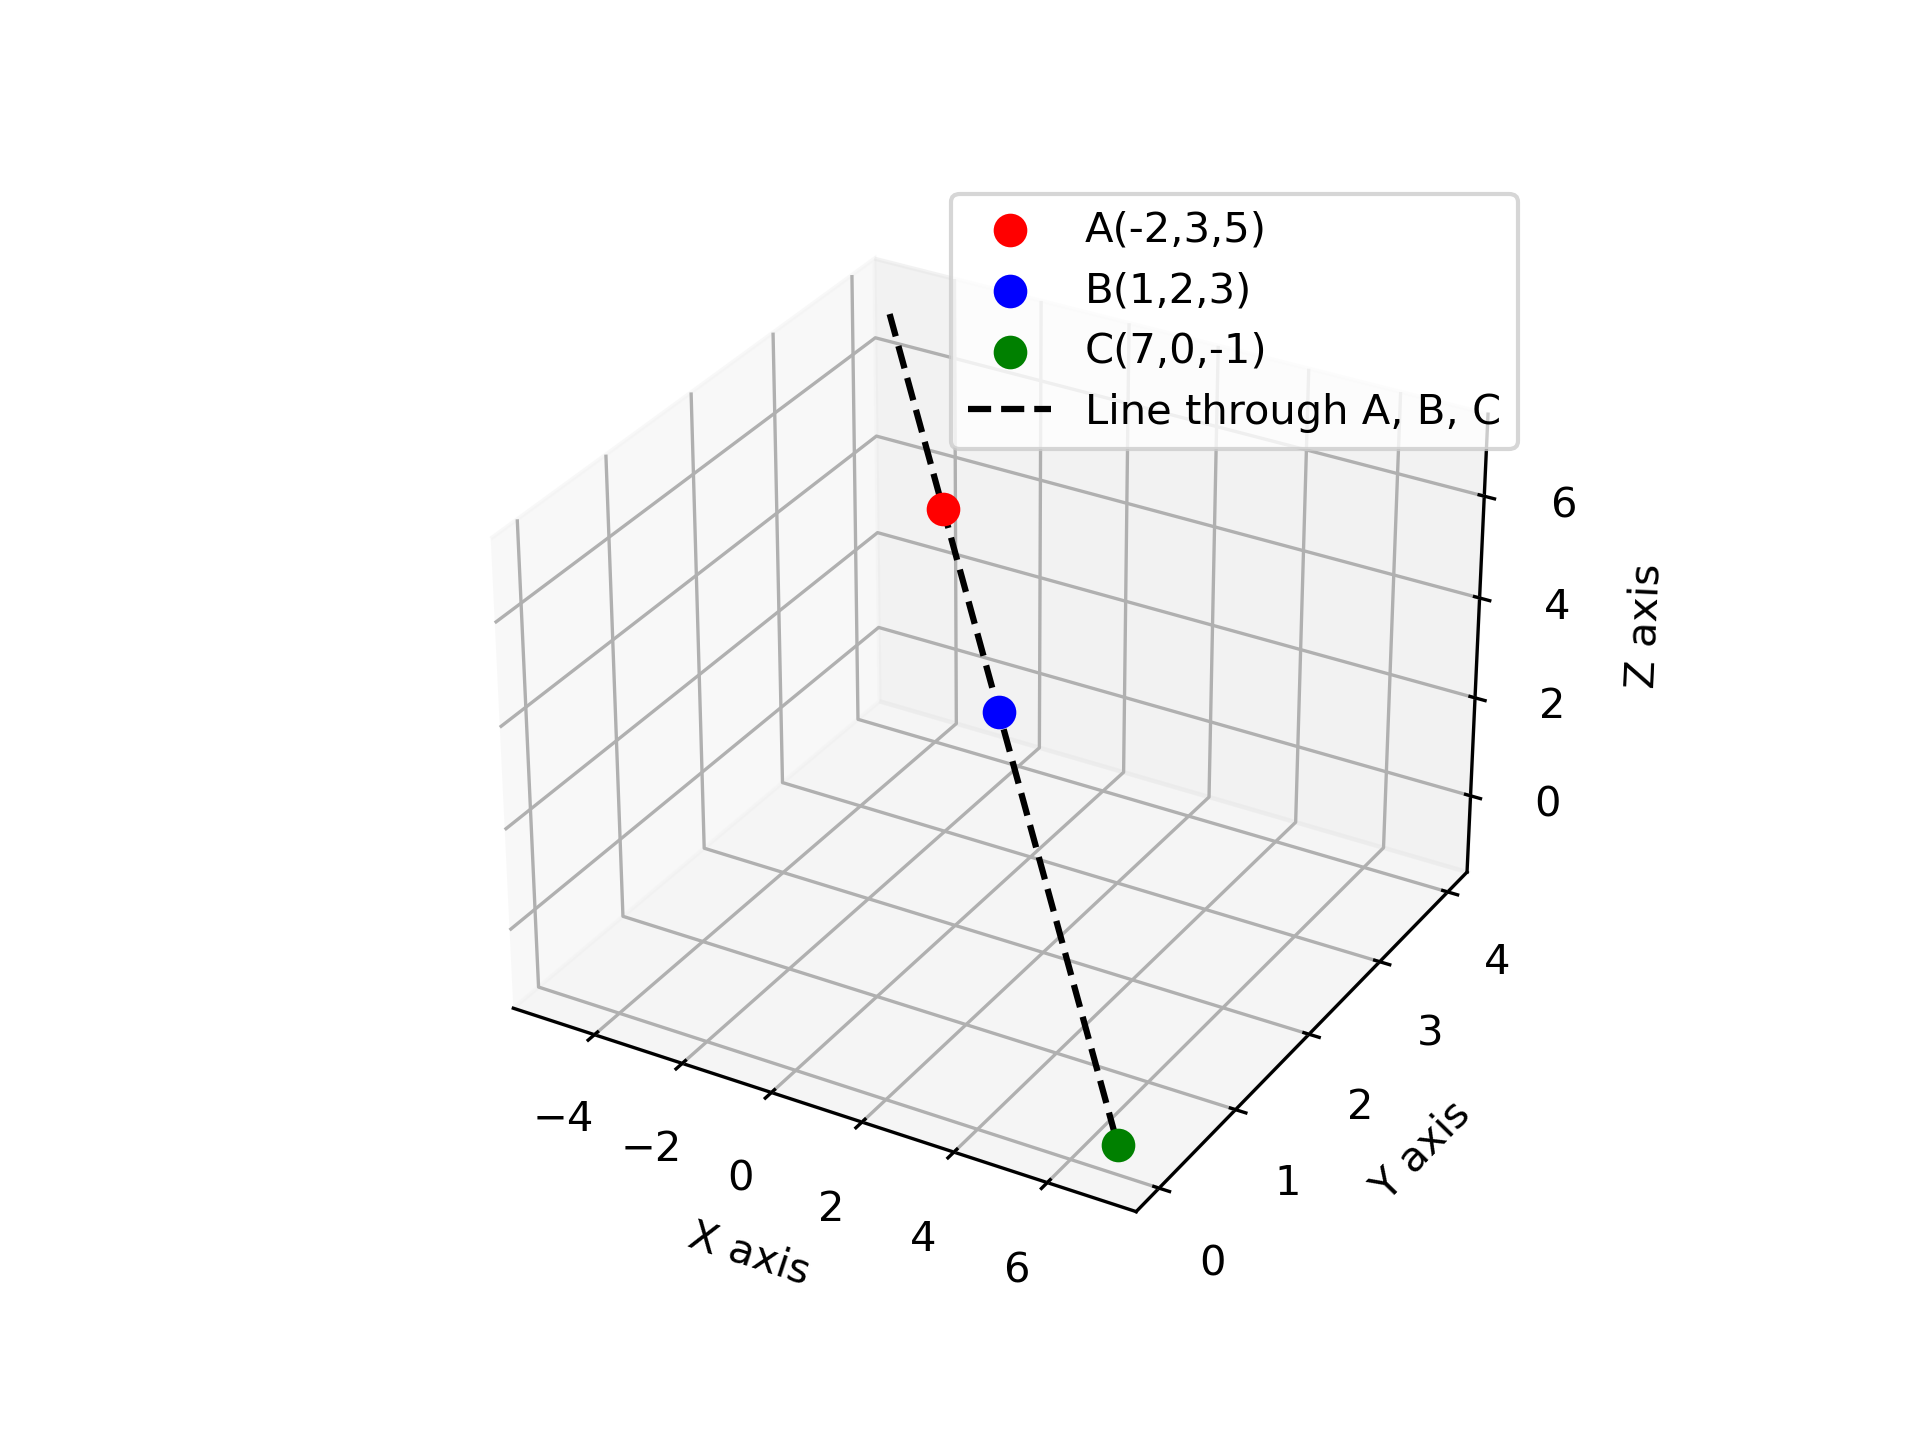
\includegraphics[width=0.6\linewidth]{/Users/unnathi/Documents/ee1030-2025/ai25btech11012/matgeo/1.11.14/figs/fig.png}
\end{center}
\end{frame}

\end{document}
